%!TEX root = ../main.tex

\section{Tree-Like Unraveling}\label{sec:unraveling}
We now describe a tree unraveling for \FGF, which we later use to construct the companion structures required in \cref{thm:main-technical-thm}.
Let $\str{A}$ be a structure with an associated binary relation $\relNext \subseteq A \times A$.
For $(e_{1}, e_{2}) \in \relNext$, we call $e_{2}$ a \emph{child} of $e_{1}$ and $e_{1}$ a $\emph{parent}$ of $e_{2}$.
A \emph{root} is an element which has no parents.
The set of $\emph{descendants}$ for an element $e$ is the smallest set which contains $e$ itself and every child of each element in the set.
The structure $\str{A}$ is a \emph{forest} if every element has at most one parent and there is at least one root.
A \emph{tree} is a forest with exactly one root.
Using the well-known unraveling for transation systems, it can be shown that every satisfiable modal logic formula is satisfiable in a tree model.
The same holds true for \FGF-formula, using the HAF-unraveling introduced by Bednarczyk~\cite[Sec 3.3]{Bednarczyk21}.
Even though the tree unraveling of a structure $\str{A}, \elemtuplea$ can be infinite for finite $\str{A}$,
for many modal logic variants, companions for a van Benthem style characterisation can be constructed based on the infinite unraveling~\cite{Otto04}.

Unfortuntately, constructing a finite version of the HAF-unraveling is not enough to prove \cref{thm:main-technical-thm}.
Consider the two finite structures shown in \cref{fig:unravel-haf}, which are both already fully HAF-unraveled, but can be distinguished by the GF sentence $\forall b,c. E(b,c) \implies \exists a. P(a,b,c)$.
This shows that even if the HAF-unraveling is finite, it does not provide GF-bisimilar companions.
\begin{figure}
  \centering
    \begin{tikzpicture}[baseline=(current bounding box.north)]
        \draw[tolbrightGreen, line cap=round, line width=2em] (-0em,8em) -- ++(0,-8em);
        \draw[tolbrightYellow, line cap=round, line width=0.5em, -{Latex[length=2em]}] (0,4em) -- (0,0em);

        \draw [black, line width=0.1em, fill=white] (0em, 8em) circle [radius=0.8em] node[anchor=center] {1};
        \draw [black, line width=0.1em, fill=white] (0em, 4em) circle [radius=0.8em] node[anchor=center] {2};
        \draw [black, line width=0.1em, fill=white] (0em, 0em) circle [radius=0.8em] node[anchor=center] {3};

        \begin{scope}[xshift=10em]
            \draw[tolbrightGreen, line cap=round, line width=2em] (-0em,8em) -- ++(0,-8em);
            \draw[tolbrightYellow, line cap=round, line width=0.5em, -{Latex[length=2em]}] (0em,4em) -> (6em,2em);
            \draw[tolbrightYellow, line cap=round, line width=0.5em, -{Latex[length=2em]}] (0,4em) -- (0,0em);

            \draw [black, line width=0.1em, fill=white] (0em, 8em) circle [radius=0.8em] node[anchor=center] {1};
            \draw [black, line width=0.1em, fill=white] (0em, 4em) circle [radius=0.8em] node[anchor=center] {2};
            \draw [black, line width=0.1em, fill=white] (0em, 0em) circle [radius=0.8em] node[anchor=center] {3};
            \draw [black, line width=0.1em, fill=white] (6em, 2em) circle [radius=0.8em] node[anchor=center] {3'};

            \node[tolbrightGreen] at (-2em, 6em) {P};
            \node[tolbrightYellow] at (-1.5em, 2em) {E};
            \node[tolbrightYellow] at (3em, 4em) {E};
        \end{scope}

        \node[font=\Large] at (5em, 4em) {$\sim_{FGF}$};

        \node[tolbrightGreen] at (-2em, 6em) {P};
        \node[tolbrightYellow] at (-1.5em, 2em) {E};
    \end{tikzpicture}%
    \caption{Two FGF-bisimilar HAFs which are not GF-bisimilar. Relations are drawn top to bottom, so the green area marks the relation $\relP(1,2,3)$}%
    \label{fig:unravel-haf}
\end{figure}
We construct an unraveling that fulfills the following theorem:
\begin{theorem}\label{thm:inf-unraveling-upgrading}
  Let $\str{A}, \elemtuplea \bisimto_{\FGF} \str{B}, \elemtupleb$ for two pointed $\sigma$-structures.
  Then there are unravelings $\unravel{A}, \elemtuptuplea$ and $\unravel{B}, \elemtuptupleb$ which are both:
  \begin{itemize}
    \item $\FGF$-similar to the original structures: $\unravel{A}, \elemtuptuplea \bisimto_{\FGF} \str{A}, \elemtuplea$ and $\unravel{B}, \elemtuptupleb \bisimto_{\FGF} \str{B}, \elemtupleb$
    \item $\GF$-bisimilar: $\unravel{A}, \elemtuptuplea \bisimto_{\GF} \unravel{B}, \elemtuptupleb$
  \end{itemize}
\end{theorem}

\noindent \textbf{Domain of the unraveling}
Let $\str{A}, \elemtuplea^{(0)}$ be a pointed $\sigma$-structure.
A \emph{bisimulation sequence} of length $\ell$ is a sequence of the form $\elemtuplea^{(0)}(i^{(1)}, j^{(1)})\elemtuplea^{(1)}\cdots(i^{(\ell)}, j^{(\ell)})\elemtuplea^{(\ell)}$, where each $a^{(k)}$ is a live tuple in $\str{A}$ and $i^{(k)}, j^{(k)}$ are indices such that $\elemtupleafromto{i^{(k)}}{j^{(k)}}^{(k-1)} = \elemtupleafromto{1}{j^{(k)}-i^{(k)}+1}^{k}$.
These bisimulation sequences arise naturally when considering bisimilar structures to $\str{A}$.
If $\str{B}, \elemtupleb^{(0)}$ is a $\sigma$-structure that is \FGF-bisimilar to $\str{A}, \elemtuplea^{(0)}$, then we can apply \ref{bisim:fforth} $\ell$ times to find tuples $\elemtupleb^{1}, \ldots, \elemtupleb^{\ell}$ for a corresponding bisimulation sequence in $\str{B}$.
Note that the infix selected by the indices $(i^{(k)}, j^{(k)})$ is not required to be maximal.
This is illustrated in the following examples of bisimulation sequences.
\begin{figure}[H]
  \centering
    \begin{minipage}[t]{0.2\textwidth}
        \raggedleft
        \vspace{0pt}
        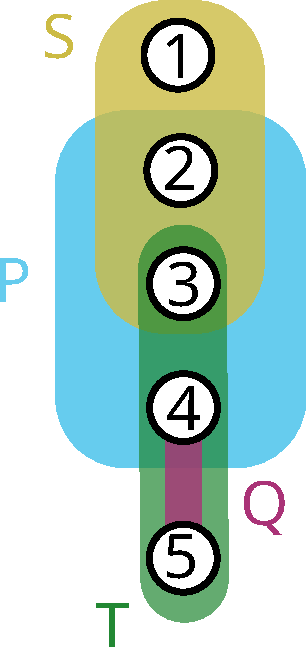
\includegraphics[scale=0.5]{res/example-struct-1}
    \end{minipage}
    \hspace{4em}
    \begin{minipage}[t]{0.6\textwidth}
      {%
      \newcommand{\tups}{{\color{tolbrightYellowDarker}\elemtuples}}%
      \newcommand{\tupp}{{\color{tolbrightCyanDarker}\elemtuplep}}%
      \newcommand{\tupt}{{\color{tolbrightGreen}\elemtuplet}}%
      \newcommand{\tupq}{{\color{tolbrightPurple}\elemtupleq}}%
      The picture on the left shows a structure with the relations: $\relS(1,2,3)$, $\relP(2,3,4)$, $\relT(3,4,5)$, $\relQ(4,5)$

      \vspace{1ex}
      Let $\tups = (1, 2, 3), \tupp = (2, 3, 4), \tupt = (3, 4, 5), \tupq = (4,5)$.

      \vspace{1ex}
      Some examples of bisimulation sequences in this structure are:
      \begin{itemize}
          \item $\tups(3,3)\tupt$
          \item $\tups(2,3)\tupp(2,3)\tupt$
      \end{itemize}

      Bisimulation sequences are not required to use maximal infixes, so the following are also valid bisimulation sequences:
      \begin{itemize}
          \item $\tups(2,2)\tupp$
          \item $\tups(3,3)\tupt(2,2)\tupq$
      \end{itemize}
      }
    \end{minipage}
    \caption{Examples for bisimulation sequences}
\end{figure}

Let $\Seq{A}$ be the set of bisimulation sequences for a structure $\str{A}$.
Consider the final tuple of a bisimulation sequence.
This tuple has a prefix of elements which are shared with the previous tuple, and a suffix of unshared elements.
We now introduce a counter to distinguish these unshared elements.
The \emph{unraveling domain} for $\str{A}$ is a set, defined as follows:
\bfside{This looks really ugly. Any way to write this in a better way?}
\begin{equation*}
\unraveldom{A} = \Seq{A} \times \mathbb{N} \setminus \left\{ (\sigma(i,j)\bar{a}, k) \colon\, k \le j-i+1\ \text{or}\ k > |a| \right\}
\end{equation*}
For an element $e \in \unraveldom{A}$ where $e = (\rho, k)$, we use the notation $\seq{e} = \rho$ and $\ctr{e} = k$ to denote the sequence and the counter of this element, respectively.
Let $\elemtuplea$ be the final tuple of $\seq{e}$, so $\seq{e} = \cdots \elemtuplea$.
Since the counter is an index into final tuple, we can define the projection $\pi(e)$ as: $\pi(e) = \elema_{\ctr{e}}$.
The unraveling domain is a forest\bfside{does this require some justification or is it obvious enough?}, with the binary relation $\relNext \subseteq \unraveldom{A} \times \unraveldom{A}$ defined such that $(s, t) \in \relNext$ iff either:
\begin{description}
  \item[\desclabel{(addCtr)}{next:addctr}] $\seq{s} = \seq{t}$, $\ctr{t} = \ctr{s} + 1$, or
  \item[\desclabel{(addSeq)}{next:addseq}] $\seq{t} = \seq{s} (i,j) \elemtuplea$ for some $i, j, \elemtuplea$ and $\ctr{s} = j, \ctr{t} = (j - i + 1) + 1$
\end{description}

\noindent
The definition of $\relNext$ has the following nice property: if $(s,t) \in \relNext$ and $t$ projects to $a_{k}$ for $k > 1$, then $s$ projects to $a_{k-1}$, where $k = \ctr{t}$ and $\elemtuplea$ is the tuple such that $\seq{t} = \cdots \elemtuplea$.
We prove this by case analysis on the two cases of $\relNext$.
The~\ref{next:addctr} case is simple: in this case $\seq{s} = \seq{t}$ and $\ctr{s} = k - 1$, so the property follows directly from the definition of $\pi$.
For the~\ref{next:addseq} case, let $\seq{t} = \seq{s} (i,j) \elemtuplea$ and $\seq{s} = \cdots \elemtupleb$.
Further, in this case $k = (j - i + 1) + 1$ and $\ctr{s} = j$.
By the fact that $\seq{t}$ is a bisimulation sequence, we know that $\elemtupleafromto{1}{j-i+1} = \elemtuplebfromto{i}{j}$.
In particular, it follows that $\pi(s) = b_{j} = a_{j-i+1} = a_{k-1}$, concluding the proof.

\noindent
\textbf{Relations in the unraveling}
A tuple of elements $(e_{1}, \ldots, e_{n})$ is a \emph{next chain} if adjacent elements are related by $\relNext$, so $(e_{i}, e_{i+1}) \in \relNext$ for all $i$.
If the length $n$ of the next chain is less than $\ctr{e_{n}}$, then we know by the previous observation that the projection of the chain is $\elemtuplee_{(\ctr{e_{n}}-n+1)\ldots{}\ctr{e_{n}}}$, where $\elemtuples$ is the final tuple of $\seq{e_{n}}$.
We define the tree unraveling such that relations are only realized by tuples which are next chains.
Additionally, we limit the length of the chain to be less than the counter of the last element of the tuple.
For this, let $\mathtt{bound}(\elemtuptupler)$ of some tuple $\elemtuptupler$ be equal to $\ctr{\elemtuptupler_{|\elemtuptupler|}}$ (the counter of the last element of the tuple).
Let $\str{A}, \elemtuplea$ be a $\sigma$-structure and $\unraveldom{A}$ be the unraveling domain.
Let $\elemtuptuplea = ((\elemtuplea, 1), \ldots, (\elemtuplea, |\elemtuplea|))$.
The \emph{tree unraveling} $\unravel{A}, \elemtuptuplea$ is the tree with root $(\elemtuplea, 1)$ and all descendants according to the relation $\relNext$.
For relations $\relR \in \sigma$, we let $\elemtuptupler \in \relR^{\unravel{A}}$ if and only if:
\begin{enumerate}
  \item $\pi[\elemtuptupler] \in \relR^{}$,
  \item $\bigwedge_{k=1}^{|\elemtuptupler|-1}{(\elemr_{k},\elemr_{k+1}) \in \relNext}$, and
  \item $|\elemtuptupler| \le \mathtt{bound}(\elemtuptupler)$
\end{enumerate}
The second and third condition restrict live tuples to be next chains with a length bounded by the counter of the last element of the tuple, as discussed before.

We illustrate the construction with an example.
Recall the left structure from \cref{fig:unravel-haf}.
Let $\elemtuplep = (1,2,3)$ and $\elemtuplee = (2,3)$.
The picture below shows the tree unraveling with root $(\elemtuplep, 1)$.
\begin{figure}[H]
  \centering
  \begin{tikzpicture}
    \draw[tolbrightGreen, line cap=round, line width=2.2em] (-0em,8em) -- ++(0,-8em);
    \draw[tolbrightYellow, line cap=round, line width=0.5em, -{Latex[length=2em]}] (0em,4em) -> (6em,1em);
    \draw[tolbrightYellow, line cap=round, line width=0.5em, -{Latex[length=2em]}] (0,4em) -- (0,0em);

    \draw [black, line width=0.1em, fill=white] (0em, 8em) ellipse (1em and 0.8em) node[anchor=center] {$(\elemtuplep, 1)$};
    \draw [black, line width=0.1em, fill=white] (0em, 4em) ellipse (1em and 0.8em) node[anchor=center] {$(\elemtuplep, 2)$};
    \draw [black, line width=0.1em, fill=white] (0em, 0em) ellipse (1em and 0.8em) node[anchor=center] {$(\elemtuplep, 3)$};
    \draw [black, line width=0.1em, fill=white] (6em, 0em) ellipse (3em and 1em) node[anchor=center] {$(\elemtuplep(2,2)\elemtuplee, 2)$};

    \node[tolbrightGreen] at (-2em, 6em) {P};
    \node[tolbrightYellow] at (-1.5em, 2em) {E};
    \node[tolbrightYellow] at (3em, 4em) {E};
  \end{tikzpicture}
\end{figure}
First, observe that the structure is isomorphic to the structure on the right in \cref{fig:unravel-haf}.
It is easy to see that the structure on the right also unravels to an isomorphic structure with this construction.
Thus, at least in this example, \cref{thm:inf-unraveling-upgrading} is not violated.
Consider the tuples $\elemtuptuplea = ((\elemtuplep, 1), (\elemtuplep, 2), (\elemtuplep, 3))$ and $\elemtuptupleb = ((\elemtuplep, 1), (\elemtuplep, 2), (\elemtuplep(2,2)\elemtuplee, 2))$.
These tuples have equal projections: $\pi(\elemtuptuplea) = \pi(\elemtuptupleb) = \elemtuplep$.
But $\elemtuptuplea \in \relP^{\unravel{A}}$ while $\elemtuptupleb \notin \relP^{\unravel{A}}$.
This is because $\mathtt{bound}(\elemtuptupleb) = 2$ and $|\elemtuptupleb| = 3$, so the bound for $\elemtuptupleb$ is not large enough.

We now prove \cref{thm:inf-unraveling-upgrading} for this unraveling.
\begin{proof}
  \bfbox{write proof}
\end{proof}
